% \begin{titlepage}
% %	\includepdf[pages=-]{front_cover.pdf}

% % The easiest way to cope with RuG font requirements is just use your favorite text editor (word, libre) and export that to PDF. Remember to set your page to B5! There's a .doc file attached.
% 	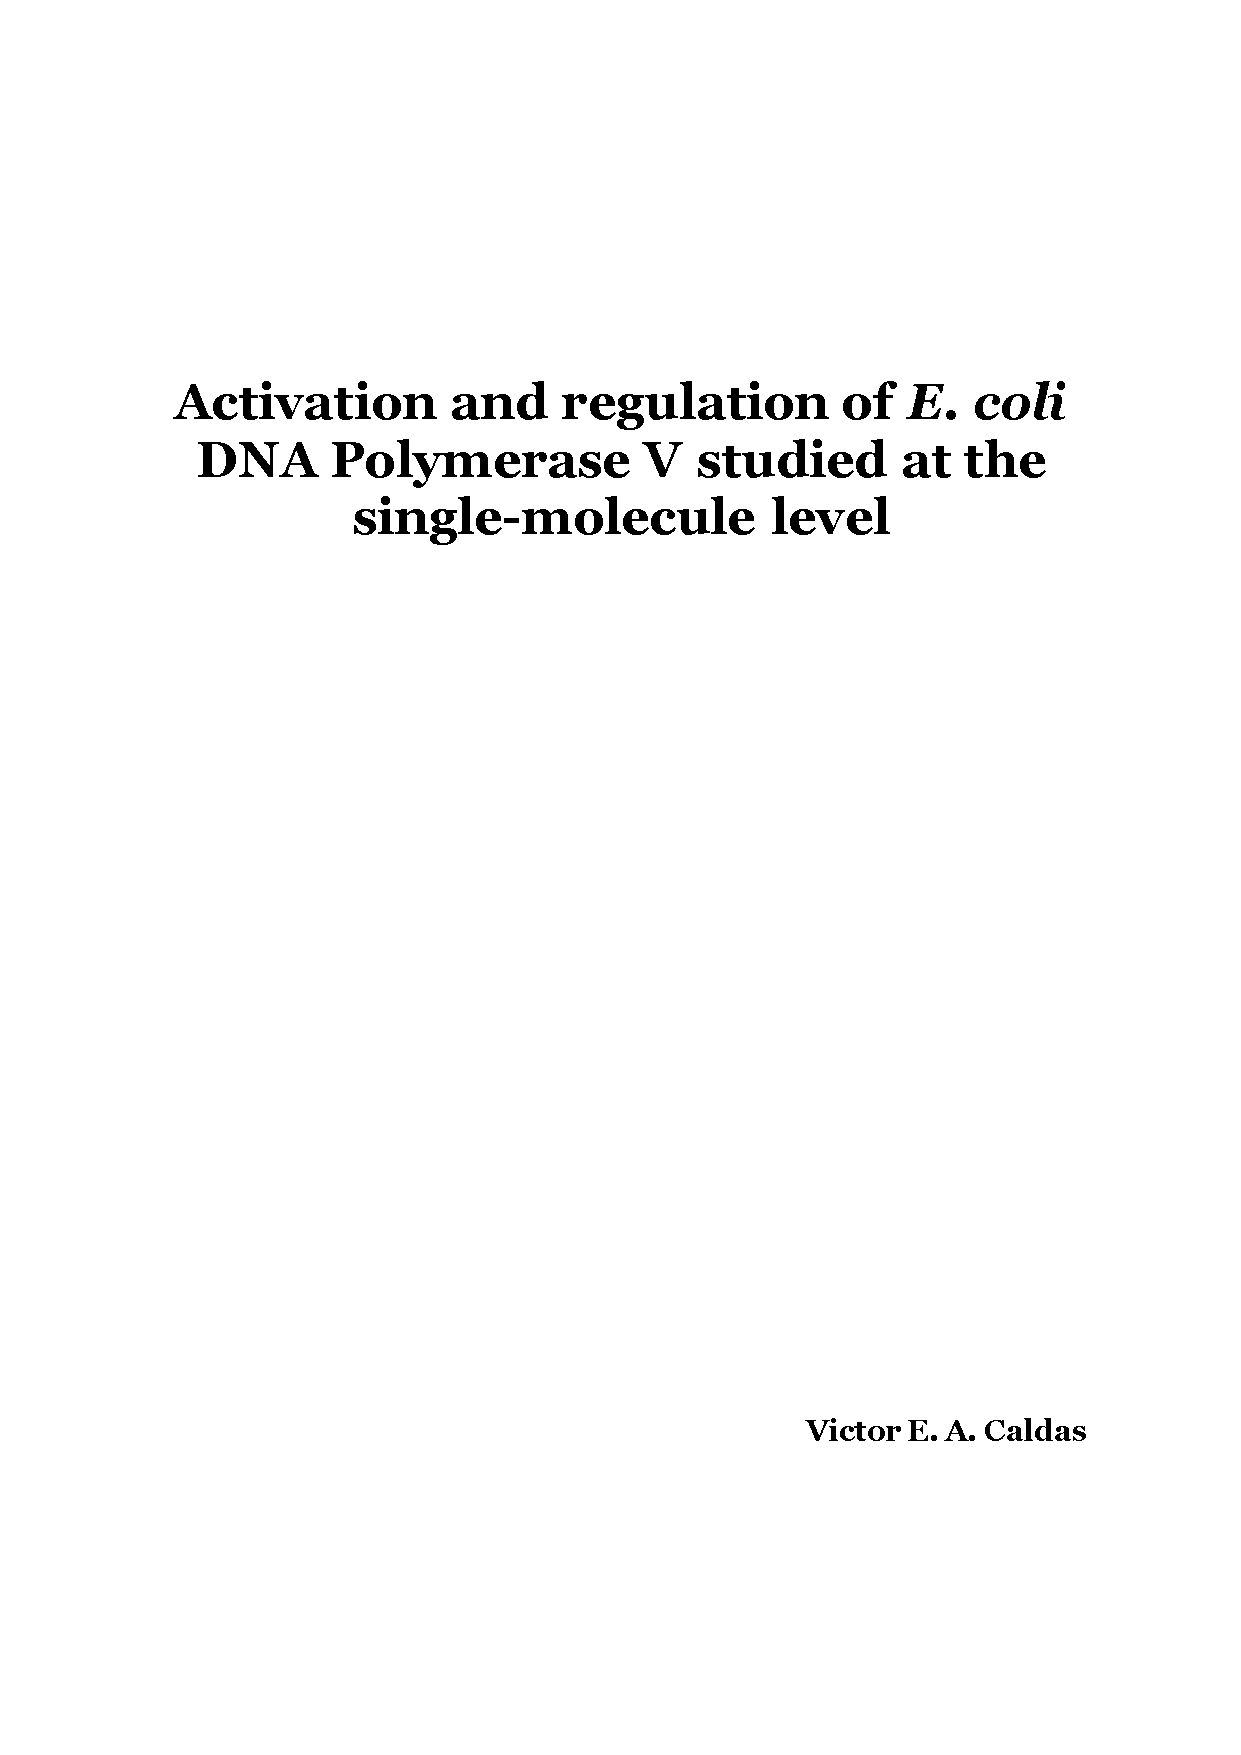
\includepdf[pages=-]{title/firstpage.pdf}
	
	
% 	%%%%%%%%%%%%%%%%%%%%%%%%%%%%% Book information page %%%%%%%%%%%%%%%%%%%%%%%%%%%%%%%%%%%%%
	
% 	\newpage \thispagestyle{empty}
% 	\vspace*{3.9cm}%{4.7cm} was 5.7, save 2 for FSC logo
	
	
% 	\begin{figure}[!h]
% 		\includegraphics[width=\textwidth]{images/frontmatter/zernike.pdf}
% 	\end{figure}
	
% 	\vfill
% 	\begin{figure}[!h]
% 		\includegraphics[width=\textwidth]{images/frontmatter/all-logos.pdf}
% 	\end{figure}
% 	\noindent
% 	{\small 
% 		Zernike Institute PhD thesis series 2016-12 \\
% 		ISSN:   1570-1530\\
% 		ISBN:	978-90-367-8806-9 \\
% 		ISBN:   978-90-367-8805-2 (electronic version) \\
% 		\\
% 		The work described in this thesis was performed in the research group Single Molecule Biophysics of the Zernike Institute for Advanced Materials at the University of Groningen, the Netherlands. \\
% 		\\
% 		Cover design: Victor E. A. Caldas\\
% 		Cover image: Super-resolution image reconstruction o \textit{E. coli} cells. Membrane marker (red) is LacY-eYFP and blue is UmuC-mKate2.
% 		\\
% 			%	An electronic version of this dissertation is available at: \\
% 	%	\url{http://MYTHESIS.COM}
% 		Printed by: GVO drukkers \& vormgevers B.V. \\
% 		} 	
	
	
% 	\clearpage
	
% 	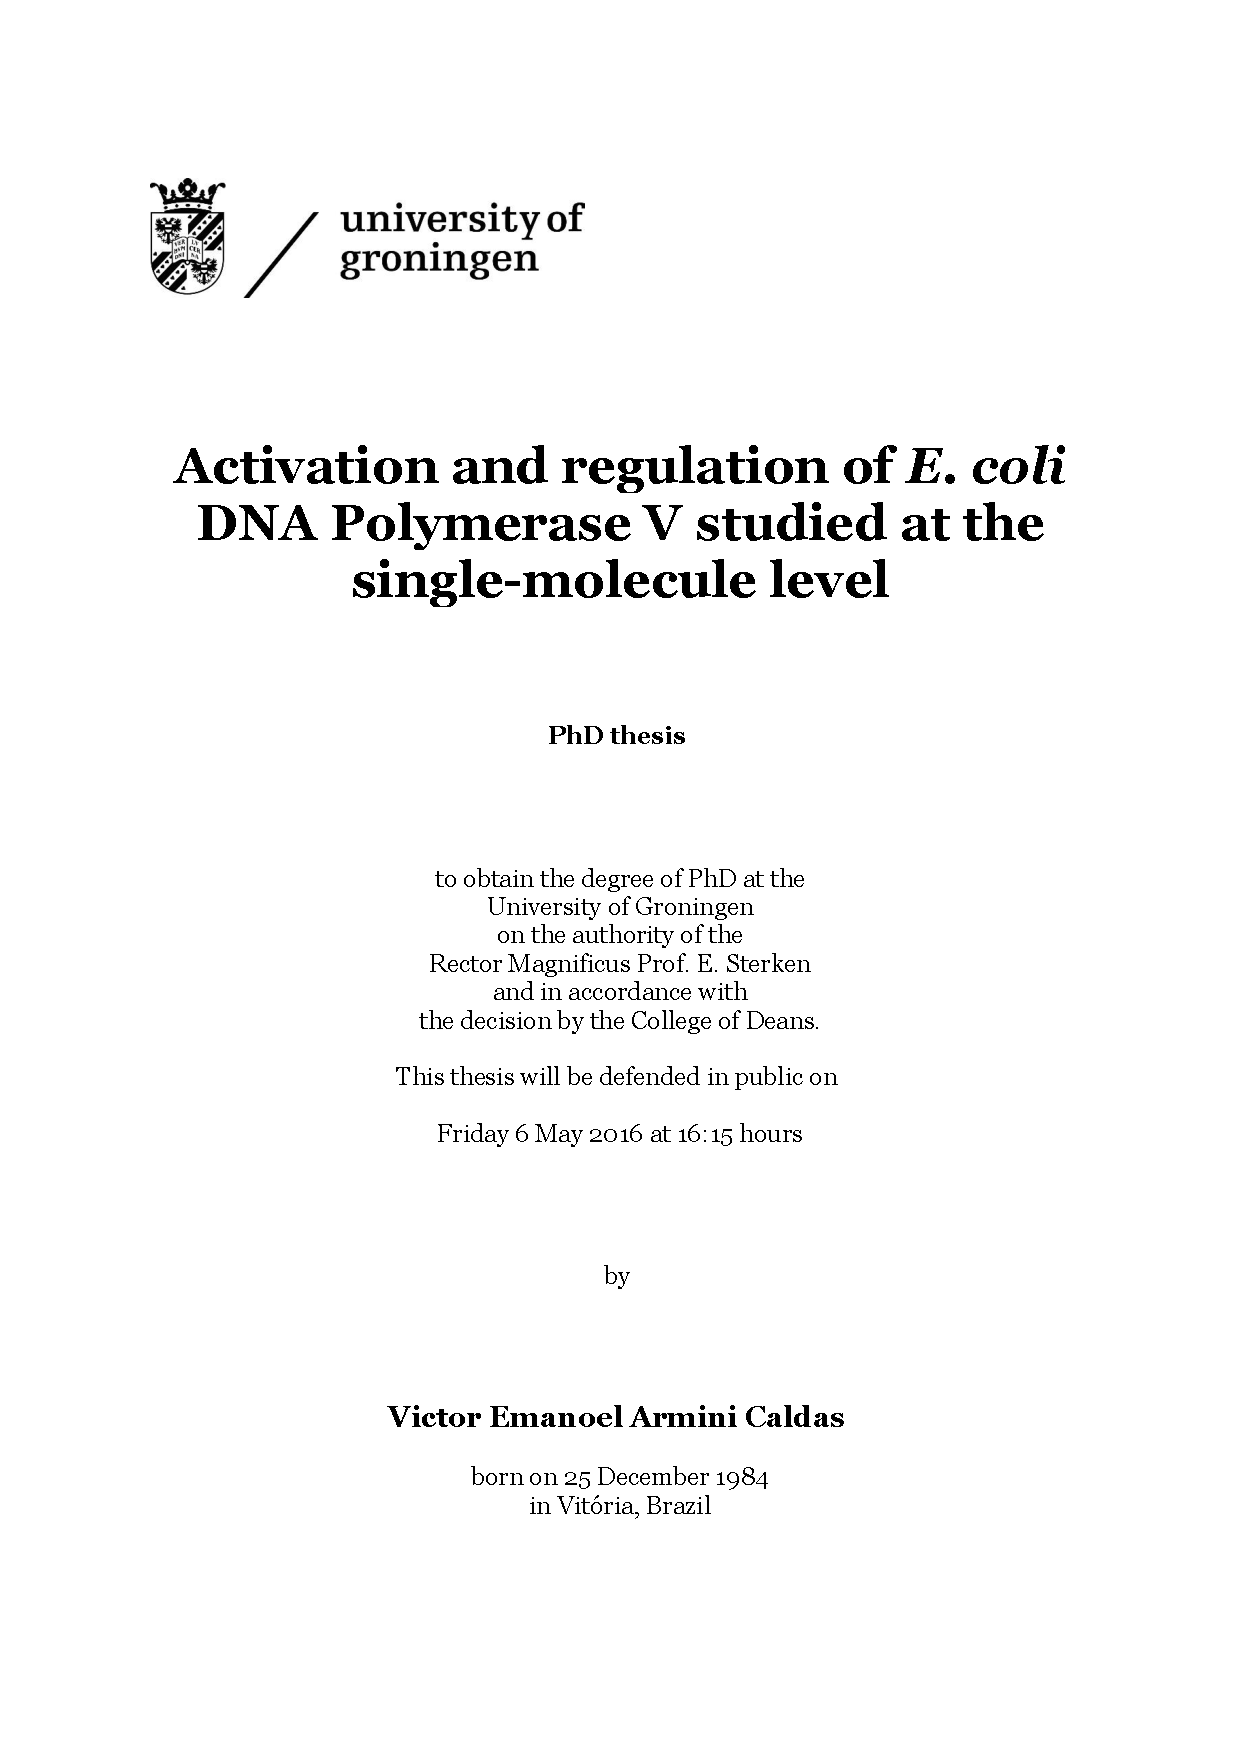
\includepdf[pages=-]{titlepage.pdf}
	
% \end{titlepage}

\begin{titlepage}

\begin{center}

%% Extra whitespace at the top.
\vspace*{2\bigskipamount}

%% Print the title.
{\makeatletter
\titlestyle\bfseries\LARGE\@title
\makeatother}

%% Print the optional subtitle.
{\makeatletter
\ifx\@subtitle\undefined\else
    \bigskip
    \titlefont\titleshape\Large\@subtitle
\fi
\makeatother}

\end{center}

\cleardoublepage
\thispagestyle{empty}
	\begin{figure}[!h]
		
\includegraphics[width=0.3\textwidth]{title/rugr_logoenv_zwart_rgb.jpeg}
	\end{figure}
\begin{center}

%% The following lines repeat the previous page exactly.

\vspace*{2\bigskipamount}

%% Print the title.
{\makeatletter
\titlestyle\bfseries\LARGE\@title
\makeatother}

%% Print the optional subtitle.
{\makeatletter
\ifx\@subtitle\undefined\else
    \bigskip
    \titlefont\titleshape\Large\@subtitle
\fi
\makeatother}

%% Uncomment the following lines to insert a vertically centered picture into
%% the title page.
%\vfill
%\includegraphics{title}
\vfill

%% Apart from the names and dates, the following text is dictated by the
%% promotieregelement.

{\Large\titlefont\bfseries PhD Thesis}

\bigskip
\bigskip

to obtain the degree of PhD at the University of Groningen
on the authority of the Rector Magnificus Prof. C. Wijmenga and in accordance with
the decision by the College of Deans.
% This thesis will be defended in public on Monday 17 January 2022 at 14.30 hours

\bigskip
\bigskip

by

\bigskip
\bigskip

%% Print the full name of the author.
\makeatletter
{\Large\titlefont\bfseries\@firstname\ \titleshape{\MakeUppercase{\@lastname}}}
\makeatother

\bigskip
\bigskip

% Master of Science in Computer Science, \\
% Technische Universität München, Duitsland,

% geboren te Schweinfurt, Duitsland.

%% Extra whitespace at the bottom.
\vspace*{2\bigskipamount}

\end{center}

\clearpage
\thispagestyle{empty}

%% The following line is dictated by the promotieregelement.
\noindent \textbf{Supervisors}

%% List the promotors (supervisors).
\medskip\noindent
\begin{tabular}{l}
    Dr.\ P.MA\ van Ooijen\\ Dr.\ M.\ Sijtsema 
    % Deursen \\
    % copromotor: Dr.\ ir.\ G.\ Gousios
\end{tabular}

\bigskip
% \noindent Samenstelling promotiecommissie:

% %% List the committee members, starting with the Rector Magnificus and the
% %% promotor(s) and ending with the reserve members.
% \medskip\noindent
% \begin{tabular}{p{4.5cm}l}
%     Rector Magnificus, & voorzitter \\
%     Prof.\ dr.\ A.\ van Deursen, & Technische Universiteit Delft \\
%     Dr.\ A.E.\ Zaidman, & Technische Universiteit Delft \\
%     Dr.\ ir.\ G.\ Gousios, & Technische Universiteit Delft \\

%     \medskip
%     \mbox{\emph{Onafhankelijke leden:}} & \\
%     Prof.\ dr.\ ir.\ G.J.P.M.\ Houben, & Technische Universiteit Delft \\
%     Prof. dr. P. Runeson, & Lund Universitet, Sweden \\
%     Dr.\ Th.\ Zimmermann, & Microsoft Research, \\ &United States of America \\
%     Prof. dr. D. Spinellis, & Athens University of Economics and Business, \\&
%     Greece \\
    
%     Prof.\ dr.\ ir.\ E.\ Visser, & Technische Universiteit Delft, reservelid \\ \\

%     \multicolumn{2}{l}{Prof. dr. D. Spinellis has contributed to the end
%     phase of writing \ldots} \\
% \end{tabular}

% %% Include the following disclaimer for committee members who have contributed
% %% to this dissertation. Its formulation is again dictated by the
% %% promotieregelement.
% %\medskip
% %\noindent  %Prof.\ Dr.\ D.\ Spinellis has contributed to the creation of this thesis.

% \medskip
% \medskip
% % TODO Include http://www.win.tue.nl/ipa/?page_id=309
% \noindent The work in the thesis has been carried out under the auspices of the research school IPA
% (Institute for Programming research and Algorithmics).

% \medskip
% %% Here you can include the logos of any institute that contributed financially
% %% to this dissertation.
% \vfill
% \begin{center}
%     
\includegraphics[height=0.5in]{title/logos/tudelft}
%     \hspace{2em}
%     %
\includegraphics[height=0.5in]{title/logos/casimir} \\
%     
\includegraphics[height=0.5in]{title/logos/nwo}
%     \\ \vspace{0.5cm}
%     
\includegraphics[height=0.5in]{title/logos/ipa}
% \end{center}
% \vfill

% \noindent
% \begin{tabular}{@{}p{0.2\textwidth}@{}p{0.8\textwidth}}
%   \textit{Keywords:} &  \\[\medskipamount]
%       \textit{Printed by:} &  \\[\medskipamount]
%       \textit{Cover:} &  \\[\medskipamount]
%       \textit{Style:} & TU Delft House Style, with modifications by Moritz Beller \\& \url{https://github.com/Inventitech/phd-thesis-template} \\[\medskipamount]
% \end{tabular}

% \medskip
% \medskip
% \noindent The author set this thesis in \LaTeX\xspace using the Libertinus and Inconsolata fonts.

% \vspace{\bigskipamount}

% Copyrighting this is stupid, questionable, and probably illegal, because large parts of the
% thesis have already been published with the copyright resigning with the publisher.
%\noindent Copyright \textcopyright\ 2015 by A.~Einstein

%% Uncomment the following lines if this dissertation is part of the Casimir PhD
%% Series, or a similar research school.
%\medskip
%\noindent Casimir PhD Series, Delft-Leiden 2015-01

%\medskip
% \noindent ISBN \ldots

% \medskip
% \noindent An electronic version of this dissertation is available at \\
% \url{http://repository.tudelft.nl/}.

\end{titlepage}
